\ifx\wholebook\relax \else

\documentclass[b5paper]{article}
\usepackage[nomarginpar
  %, margin=.5in
]{geometry}

\addtolength{\oddsidemargin}{-0.05in}
\addtolength{\evensidemargin}{-0.05in}
\addtolength{\textwidth}{0.1in}

\usepackage[en]{../../../prelude}

\setcounter{page}{1}

\begin{document}

\title{Radix tree}

\author{Xinyu LIU
\thanks{{\bfseries Xinyu LIU} \newline
  Email: liuxinyu95@gmail.com \newline}
  }

\maketitle
\fi

\markboth{Radix tree}{Elementary algorithms}

\ifx\wholebook\relax
\chapter{Radix tree}
\numberwithin{Exercise}{chapter}
\fi

%\section{Introduction}
\label{introduction} \index{Radix tree}

Binary search tree stores data in nodes. Can we use the edges to carry information? Radix trees, including trie, prefix tree, and suffix tree are the data structures developed based on this idea in 1960s. They are widely used in compiler design\cite{okasaki-int-map}, and bio-information processing, like DNA pattern matching \cite{wiki-suffix-tree}.

\begin{figure}[htbp]
  \centering
  \includegraphics[scale=0.4]{img/radix-tree}
  \caption{Radix tree.}
  \label{fig:radix-tree}
\end{figure}

\Cref{fig:radix-tree} shows a Radix tree. It contains bits 1011, 10, 011, 100 and 0. When lookup a key $k=(b_0b_1...b_n)_2$, we take the first bit $b_0$ (MSB from left), check whether it is 0 or 1. For 0, turn left, else turn right. Then take the second bit and repeat looking up till either reach a leaf node or consume all the $n$ bits. We needn't store keys in Radix tree node. The information is represented by edges. The nodes labelled with key in \cref{fig:radix-tree} are for illustration purpose. If the keys are integers, we can represent them in binary format, and implement lookup with bit-wise manipulations.

\section{Integer trie}
\label{int-trie} \index{Integer trie}

We call the data structure in \cref{fig:radix-tree} \emph{binary trie}. Trie was developed by Edward Fredkin in 1960. It comes from ``re\textbf{trie}val'', pronounce as /'tri:/ by Freddkin, while others pronounce it as /'trai/ ``try''\cite{wiki-trie}. Although it's also called prefix tree in some context, we treat trie and prefix tree different in this chapter. A binary trie is a special binary tree in which the placement of each key is controlled by its bits, each 0 means `go left' and each 1 means `go right'\cite{okasaki-int-map}. Consider the binary trie in \cref{fig:big-endian-trie}. The three keys are different bit strings of ``11'', ``011'', and ``0011'' although they are all equal to 3.

\begin{figure}[htbp]
  \centering
  \includegraphics[scale=0.4]{img/big-endian-trie}
  \caption{A big-endian trie.}
  \label{fig:big-endian-trie}
\end{figure}

It is inefficient to treat the prefix zeros as valid bits. For 32 bits integers, we need a tree of 32 levels to insert number 1. Okasaki suggested to use little-endian integers instead\cite{okasaki-int-map}. 1 is represented as bits $(1)_2$, 2 as $(01)_2$, and 3 is $(11)_2$, ...

\subsection{Definition}
We can re-use binary tree structure to define the little-endian binary trie. A node is either empty, or a branch containing the left, right sub-trees, and an optional value. The left sub-tree is encoded as 0 and the right sub-tree is encoded as 1.

\lstset{frame = single}
\begin{Haskell}
data IntTrie a = Empty | Branch (IntTrie a) (Maybe a) (IntTrie a)
\end{Haskell}

Given a node in the binary trie, the integer key bound to it is uniquely determined through its position. That is the reason we need not save the key, but only the value in the node. The type of the key is always integer, we call the tree $IntTrie\ A$ if the value is of type $A$.

\subsection{Insert}
\index{Integer trie!insert}

When insert an integer key $k$ and a value $x$, we convert $k$ into binary form. If $k$ is even, the lowest bit is 0, we recursively insert to the left sub-tree; otherwise if $k$ is odd, the lowest bit is 1, we recursively insert to the right. We next divide $k$ by 2 to remove the lowest bit. For none empty trie $T = (l, v, r)$, where $l, r$ are the left and right sub-trees, and $v$ is the optional value, function $insert$ can be defined as below:

\be
\begin{array}{rcl}
insert\ k\ x\ \nil & = & insert\ k\ x\ (\nil, \textit{Nothing}, \nil) \\
insert\ 0\ x\ (l, v, r) & = & (l, \textit{Just}\ x, r) \\
insert\ k\ x\ (l, v, r) & = & \begin{cases}
  even(k): & (insert\ \dfrac{k}{2}\ x\ l, v, r) \\
  odd(k) : & (l, v, insert\ \lfloor \dfrac{k}{2} \rfloor\ x\ r) \\
\end{cases}
\end{array}
\ee

If $k = 0$, we put $x$ in the node. When $T = \nil$, it becomes $(\nil, \textit{Just}\ x, \nil)$. As far as $k \neq 0$, we goes down along the tree based on the parity of $k$. We create empty leaf $(\nil, \textit{Nothing}, \nil)$ whenever meet $\nil$ node. This algorithm overrides the value if $k$ already exists. Alternatively, we can store a list, and append $x$ to it. \Cref{fig:int-trie} shows an example trie, generated by inserting the key-value pairs of \{$ 1 \rightarrow a, 4 \rightarrow b, 5 \rightarrow c, 9 \rightarrow d$\}. Below is the example program implements $insert$:

\begin{figure}[htbp]
  \centering
  \includegraphics[scale=0.5]{img/int-trie}
  \caption{A little-endian integer binary trie of
          \{$ 1 \rightarrow a, 4 \rightarrow b, 5 \rightarrow c, 9 \rightarrow d$\}.}
  \label{fig:int-trie}
\end{figure}

\begin{Haskell}
insert k x Empty = insert k x (Branch Empty Nothing Empty)
insert 0 x (Branch l v r) = Branch l (Just x) r
insert k x (Branch l v r) | even k    = Branch (insert (k `div` 2) x l) v r
                          | otherwise = Branch l v (insert (k `div` 2) x r)
\end{Haskell}

We can define the even/odd testing by modular 2, and check if the remainder is 0 or not: $even(k) = (k \bmod 2 = 0)$. Or use bit-wise operation in some environment, like \texttt{(k \& 0x1) == 0}. We can eliminate the recursion through loops to realize an iterative implementation as below:

\begin{algorithmic}[1]
\Function{Insert}{$T, k, x$}
  \If{$T =$ NIL}
    \State $T \gets$ \Call{Empty-Node}{}  \Comment{(NIL, Nothing, NIL)}
  \EndIf
  \State $p \gets T$
  \While{$k \neq 0$}
    \If{\Call{Even?}{$k$}}
      \If{\Call{Left}{$p$} = NIL}
        \State \Call{Left}{$p$} $\gets$ \Call{Empty-Node}{}
      \EndIf
      \State $p \gets$ \Call{Left}{$p$}
    \Else
      \If{\Call{Right}{$p$} = NIL}
        \State \Call{Right}{$p$} $\gets$ \Call{Empty-Node}{}
      \EndIf
      \State $p \gets$ \Call{Right}{$p$}
    \EndIf
    \State $k \gets \lfloor k/2 \rfloor$
  \EndWhile
  \State \Call{Value}{$p$} $\gets x$
  \State \Return $T$
\EndFunction
\end{algorithmic}

\textproc{Insert} takes, a trie $T$, a key $k$, and a value $x$. For integer $k$ with $m$ bits in binary, it goes into $m$ levels of the trie. The performance is bound to $O(m)$. We design $insert\ k\ x\ T$ and \textproc{Insert}($T, k, x$) symmetric, apply $foldr$ to the former, and $foldl$ (or for-loops) to the latter to convert a list of key-value pairs to tree. For example:

\be
fromList = foldr\ (uncurry\ insert)\ \nil
\ee

The usage is $fromList$\ [(1, a), (4, b), (5, c), (9, d)], where $uncurry$ is the revert of Currying, it unpack a pair and feed to $insert$:

\be
uncurry\ f\ (a, b) = f\ a\ b
\ee

\subsection{Lookup}
\index{Integer trie!lookup}

When look up key $k$ in a none empty integer trie, if $k = 0$, then the root node is the target. Otherwise, we check the lowest bit, then recursively look up the left or right sub-tree accordingly.

\be
\begin{array}{rcl}
lookup\ k\ \nil & = & \textit{Nothing} \\
lookup\ 0\ (l, v, r) & = & v \\
lookup\ k\ (l, v, r) & = & \begin{cases}
  even(k): & lookup\ \dfrac{k}{2}\ l \\
  odd(k):  & lookup\ \lfloor \dfrac{k}{2} \rfloor\ r \\
\end{cases}
\end{array}
\ee

We can eliminate the recursion to implement the iterative $lookup$ as the following:

\begin{algorithmic}[1]
\Function{Lookup}{$T, k$}
  \While{$k \neq 0$ and $T \neq $NIL}
    \If{ \Call{Even?}{$k$} }
      \State $T \gets$ \Call{Left}{$T$}
    \Else
      \State $T \gets$ \Call{Right}{$T$}
    \EndIf
    \State $k \gets \lfloor k/2 \rfloor$
  \EndWhile
  \If{$T \neq $ NIL}
    \State \Return \Call{Value}{$T$}
  \Else
    \State \Return NIL \EndIf
\EndFunction
\end{algorithmic}

The $lookup$ function is bound to $O(m)$ time, where $m$ is the number of bits of $k$.

\begin{Exercise}\label{ex:int-trie-empty-node}
\Question{Can we change the definition from \texttt{Branch (IntTrie a) (Maybe a) (IntTrie a)} to \texttt{Branch (IntTrie a) a (IntTrie a)}, and return \textit{Nothing} if the value does not exist, and \textit{Just\ v} otherwise?}
\end{Exercise}

\begin{Answer}[ref = {ex:int-trie-empty-node}]
\Question{Can we change the definition from \texttt{Branch (IntTrie a) (Maybe a) (IntTrie a)} to \texttt{Branch (IntTrie a) a (IntTrie a)}, and return \textit{Nothing} if the value does not exist, and \textit{Just\ v} otherwise?

Besides $lookup$, we need handle branch node without value when $insert$, as the blank circle nodes in \cref{fig:int-trie}. Alternatively, we can add an additional constructor in the algebraic data type (ADT) to replace the Maybe type:

\begin{Haskell}
data IntTrie a = Empty
               | Branch (IntTrie a) a (IntTrie a)
               | EmptyBranch (IntTrie a) (IntTrie a)
\end{Haskell}
}
\end{Answer}

\section{Integer prefix tree}
\label{int-patricia} \index{Integer Patricia} \index{Integer prefix tree}

Trie is not space efficient. As shown in \cref{fig:int-trie}, there are only 4 nodes with value, while the rest 5 are empty. The space usage is less than 50\%. To improve the efficiency, we can consolidate the chained nodes to one. Integer prefix tree is such a data structure developed by Donald R. Morrison in 1968. He named it as `Patricia', standing for \textbf{P}ractical \textbf{A}lgorithm \textbf{T}o \textbf{R}etrieve \textbf{I}nformation \textbf{C}oded \textbf{I}n \textbf{A}lphanumeric\cite{patricia-morrison}. When the keys are integer, we call it integer prefix tree or simply integer tree when the context is clear. Okasaki provided the implementation in \cite{okasaki-int-map}. Consolidate the chained nodes in \cref{fig:int-trie}, we obtained an integer tree as shown in \cref{fig:little-endian-patricia}. The key to the branch node is the longest common prefix for its descendant trees. In other words, the sibling sub-trees branch out at the bit where ends at their longest prefix. As the result, integer tree eliminates the redundant spaces in trie.

\begin{figure}[htbp]
  \centering
  \includegraphics[scale=0.5]{img/little-endian-patricia}
  \caption{Little endian integer tree for the map
     \{$ 1 \rightarrow a, 4 \rightarrow b, 5 \rightarrow c, 9 \rightarrow d$\}.}
  \label{fig:little-endian-patricia}
\end{figure}

\subsection{Definition}

Integer prefix tree is a special binary tree. It is either empty $\nil$, or a leaf node of as $(k, v)$, that contains an integer key $k$ and a value $v$; or a branch with the left and right sub-trees, that share the \textbf{longest common prefix} bits for their keys. For the left sub-tree, the next bit is 0, for the right, it is 1. Denoted as $(p, m, l, r)$. Below example program defines the integer prefix tree. The branch node contains 4 components: The longest prefix $p$, a mask integer $m$ indicating from which bit the sub-trees branch out, the left and right sub-trees $l$ and $r$. The mask is $m = 2^n$ for some integer $n \geq 0$. All bits that are lower than $n$ do not belong to the common prefix.

\begin{Haskell}
data IntTree a = Empty
               | Leaf Int a
               | Branch Int Int (IntTree a) (IntTree a)
\end{Haskell}

\subsection{Insert}
\index{Integer tree!insert}
When insert integer $y$ to tree $T$, if $T$ is empty, we create a leaf of $y$; If $T$ is a singleton leaf of $x$, besides the new leaf of $y$, we need create a branch node, set $x$ and $y$ as the two sub-trees. To determine whether $y$ is on the left or right, we need find the longest common prefix $p$ of $x$ and $y$. For example if $x = 12 = (1100)_2$, $y = 15 = (1111)_2$, then $p = (11oo)_2$, where $o$ denotes the bits we don't care. We can use another integer $m$ to mask those bits. In this example, $m = 4 = (100)_2$. The next bit after $p$ presents $2^1$. It is 0 in $x$, 1 in $y$. Hence, we set $x$ as the left sub-tree and $y$ as the right, as shown in \cref{fig:int-patricia-insert-b}.

\begin{figure}[htbp]
  \centering
  \includegraphics[scale=0.7]{img/int-patricia-insert-b}
  \caption{Left: $T$ is a leaf of 12; Right: After insert 15.}
  \label{fig:int-patricia-insert-b}
\end{figure}

If $T$ is neither empty nor a leaf, we firstly check if $y$ matches the longest common prefix $p$ in the root, then recursively insert it to the sub-tree according to the next bit after $p$. For example, when insert $y = 14 = (1110)_2$ to the tree shown in \cref{fig:int-patricia-insert-b}, since $p = (11oo)_2$ and the next bit (the bit of $2^1$) is 1, we recursively insert $y$ to the right sub-tree. If $y$ does not match $p$ in the root, we need branch a new leaf as shown in \cref{fig:int-patricia-insert-c}.

\begin{figure}[htbp]
  \centering
  \subcaptionbox{Insert $14 = (1110)_2$, which matches $p = (1100)_2$. It is inserted to the right.}{\includegraphics[scale=0.5]{img/int-patricia-insert-c}}\\
  \subcaptionbox{Insert $5 = (101)_2$, which does not match $p = (1100)_2$. Branch out a new leaf.}{\includegraphics[scale=0.5]{img/int-patricia-insert-d}}
  \caption{The tree is a branch node.}
  \label{fig:int-patricia-insert-c}
\end{figure}

For integer key $k$ and value $v$, let $(k, v)$ be the leaf. For branch node, denote it as $(p, m, l, r)$, where $p$ is the longest common prefix, $m$ is the mask, $l$ and $r$ are the left and right sub-trees. Below $insert$ function defines the above 3 cases:

\be
\resizebox{\textwidth}{!}{\ensuremath{
\begin{array}{rcl}
insert\ k\ v\ \nil & = & (k, v) \\
insert\ k\ v\ (k, v') & = & (k, v) \\
insert\ k\ v\ (k', v') & = & join\ k\ (k, v)\ k'\ (k', v') \\
insert\ k\ v\ (p, m, l, r) & = & \begin{cases}
  match(k, p, m): & \begin{cases}
    zero(k, m): & (p, m, insert\ k\ v\ l, r) \\
    otherwise:  & (p, m, l, insert\ k\ v\ r) \\
  \end{cases} \\
  otherwise: & join\ k\ (k, v)\ p\ (p, m, l, r) \\
\end{cases} \\
\end{array}
}}
\ee

We create a leaf of $(k, v)$ when $T = \nil$, override the value for the same key. Function $match(k, p, m)$ tests if integer $k$ and prefix $p$ have the same bits after masked with $m$ through: $mask(k, m) = p$, where $mask(k, m) = \overline{m-1} \& k$. It applies bit-wise not to $m-1$, then does bit-wise and with $k$. $zero(k, m)$ tests the next bit in $k$ masked with $m$ is 0 or not. We shift $m$ one bit to right, then do bit-wise and with $k$:

\be
zero(k, m) = x \& (m \gg 1)
\ee

Function $join(p_1, T_1, p_2, T_2)$ takes two different prefixes and trees. It extracts the longest common prefix of $p_1$ and $p_2$ as $(p, m) = LCP(p_1, p_2)$, creates a new branch node, then set $T_1$ and $T_2$ as the two sub-trees:

\be
join(p_1, T_1, p_2, T_2) = \begin{cases}
  zero(p_1, m): & (p, m, T_1, T_2) \\
  otherwise: & (p, m, T_2, T_1) \\
\end{cases}
\ee

To calculate the longest common prefix, we can firstly compute bit-wise exclusive-or for $p1$ and $p2$, then count the highest bit $highest(xor(p_1, p_2))$ as:

\[
\begin{array}{rcl}
highest(0) & = & 0 \\
highest(n) & = & 1 + highest(n >> 1) \\
\end{array}
\]

Then generate a mask $m = 2^{highest(xor(p_1,p_2))}$. The longest common prefix $p$ can be given by masking the bits with $m$ for either $p_1$ or $p_2$, like $p = mask(p_1, m)$. The following example program implements the $insert$ function:

\begin{Haskell}
insert k x t
   = case t of
       Empty -> Leaf k x
       Leaf k' x' -> if k == k' then Leaf k x
                     else join k (Leaf k x) k' t
       Branch p m l r
          | match k p m -> if zero k m
                           then Branch p m (insert k x l) r
                           else Branch p m l (insert k x r)
          | otherwise -> join k (Leaf k x) p t

join p1 t1 p2 t2 = if zero p1 m then Branch p m t1 t2
                                else Branch p m t2 t1
    where
      (p, m) = lcp p1 p2

lcp p1 p2 = (p, m) where
    m = bit (highestBit (p1 `xor` p2))
    p = mask p1 m

highestBit x = if x == 0 then 0 else 1 + highestBit (shiftR x 1)

mask x m = x .&. complement (m - 1)

zero x m = x .&. (shiftR m 1) == 0

match k p m = (mask k m) == p
\end{Haskell}

We can also implement $insert$ imperatively:

\begin{algorithmic}[1]
\Function{Insert}{$T, k, v$}
  \If{$T = $ NIL}
    \State \Return \Call{Create-Leaf}{$k, v$}
  \EndIf
  \State $y \gets T$
  \State $p \gets$ NIL
  \While{$y$ is not leaf, and \textproc{Match}($k$, \Call{Prefix}{$y$}, \Call{Mask}{$y$})}
    \State $p \gets y$
    \If{\textproc{Zero?}($k$, \Call{Mask}{$y$})}
      \State $y \gets$ \Call{Left}{$y$}
    \Else
      \State $y \gets$ \Call{Right}{$y$}
    \EndIf
  \EndWhile
  \If{$y$ is leaf, and $k = $ \Call{Key}{$y$}}
    \State \Call{Value}{$y$} $\gets v$
  \Else
    \State $z \gets$ \textproc{Branch}($y$, \Call{Create-Leaf}{$k, v$})
    \If{$p = $ NIL}
      \State $T \gets z$
    \Else
      \If{\Call{Left}{$p$} $ = y$}
        \State \Call{Left}{$p$} $\gets z$
      \Else
        \State \Call{Right}{$p$} $\gets z$
      \EndIf
    \EndIf
  \EndIf
  \State \Return $T$
\EndFunction
\end{algorithmic}

Where \textproc{Branch}($T_1, T_2$) creates a new branch node, extracts the longest common prefix, then sets $T_1$ and $T_2$ as the two sub-trees.

\begin{algorithmic}[1]
\Function{Branch}{$T_1, T_2$}
  \State $T \gets$ \Call{Empty-Node}{}
  \State (\Call{Prefix}{$T$}, \Call{Mask}{$T$}) $\gets$ \textproc{LCP}(\Call{Prefix}{$T_1$}, \Call{Prefix}{$T_2$})
  \If{\textproc{Zero?}(\Call{Prefix}{$T_1$}, \Call{Mask}{$T$})}
    \State \Call{Left}{$T$} $\gets T_1$
    \State \Call{Right}{$T$} $\gets T_2$
  \Else
    \State \Call{Left}{$T$} $\gets T_2$
    \State \Call{Right}{$T$} $\gets T_1$
  \EndIf
  \State \Return $T$
\EndFunction
\Statex
\Function{Zero?}{$x, m$}
  \State \Return $(x \& \lfloor \dfrac{m}{2} \rfloor) = 0$
\EndFunction
\end{algorithmic}

Function \textproc{LCP} find the longest bit prefix from two integers:

\begin{algorithmic}[1]
\Function{LCP}{$a, b$}
  \State $d \gets xor(a, b)$
  \State $m \gets 1$
    \While{$d \neq 0$}
    \State $d \gets \lfloor \dfrac{d}{2} \rfloor$
    \State $m \gets 2m$
  \EndWhile
  \State \Return (\Call{MaskBit}{$a, m$}, $m$)
\EndFunction
\Statex
\Function{MaskBit}{$x, m$}
  \State \Return $x \& \overline{m - 1}$
\EndFunction
\Statex
\end{algorithmic}

\Cref{fig:int-patricia-haskell-insert} gives an example integer tree created from the $insert$ algorithm. Although integer prefix tree consolidates the chained nodes, the operation to extract the longest common prefix need linear scan the bits. For integer of $m$ bits, the insert is bound to $O(m)$.

\begin{figure}[htbp]
  \centering
  \includegraphics[scale=0.6]{img/int-patricia-haskell-insert}
  \caption{Insert $\{1 \rightarrow x, 4 \rightarrow y, 5 \rightarrow z\}$ to the big-endian integer tree.}
  \label{fig:int-patricia-haskell-insert}
\end{figure}


\subsection{Lookup}
\index{Integer tree!lookup}

When lookup key $k$, if the integer tree $T = \nil$ or it is a leaf of $T = (k', v)$ with different key, then $k$ does not exist; if $k = k'$, then $v$ is the result; if $T = (p, m, l, r)$ is a branch node, we need check if the common prefix $p$ matches $k$ under the mask $m$, then recursively lookup the sub-tree $l$ or $r$ upon next bit. If fails to match the common prefix $p$, then $k$ does not exist.

\be
\begin{array}{rcl}
lookup\ k\ \nil & = & \textit{Nothing} \\
lookup\ k\ (k', v) & = & \begin{cases}
  k = k': & \textit{Just}\ v \\
  otherwise: & \textit{Nothing} \\
  \end{cases} \\
lookup\ k\ (p, m, l, r) & = & \begin{cases}
  match(k, p, m): & \begin{cases}
    zero(k, m): & lookup\ k\ l \\
    otherwise: &  lookup\ k\ r \\
    \end{cases} \\
  otherwise: & \textit{Nothing} \\
  \end{cases}\\
\end{array}
\ee

We can also eliminate the recursion to implement the iterative lookup algorithm.

\begin{algorithmic}[1]
\Function{Look-Up}{$T, k$}
  \If{$T =$ NIL}
    \State \Return NIL
  \EndIf
  \While{$T$ is not leaf, and \textproc{Match}($k$, \Call{Prefix}{$T$}, \Call{Mask}{$T$})}
    \If{\textproc{Zero?}($k$, \Call{Mask}{$T$})}
      \State $T \gets$ \Call{Left}{$T$}
    \Else
      \State $T \gets$ \Call{Right}{$T$}
    \EndIf
  \EndWhile
  \If{$T$ is leaf, and \Call{Key}{$T$} $=k$}
    \State \Return \Call{Value}{$T$}
  \Else
    \State \Return NIL
  \EndIf
\EndFunction
\end{algorithmic}

The $lookup$ algorithm is bound to $O(m)$, where $m$ is the number of bits in the key.

\begin{Exercise}\label{ex:int-tree-lookup}
\Question{Write a program to implement the $lookup$ function.}
\Question{Implement the pre-order traverse for both integer trie and integer tree. Only output the keys when the nodes store values. What pattern does the result follow?}
\end{Exercise}

\begin{Answer}[ref = {ex:int-tree-lookup}]
\Question{Write a program to implement the $lookup$ function.

\begin{Haskell}
import Data.Bits

type Key = Int
type Prefix = Int
type Mask = Int

data IntTree a = Empty
               | Leaf Key a
               | Branch Prefix Mask (IntTree a) (IntTree a)

lookup :: Key -> IntTree a -> Maybe a
lookup _ Empty = Nothing
lookup k (Leaf k' v) = if k == k' then Just v else Nothing
lookup k (Branch p m l r) | match k p m = if zero k m then lookup k l
                                          else lookup k r
                          | otherwise = Nothing

match :: Key -> Prefix -> Mask -> Bool
match k p m = (mask k m) == p

mask :: Int -> Mask -> Int
mask x m = (x .&. complement (m - 1))

zero :: Int -> Mask -> Bool
zero x m = x .&. (shiftR m 1) == 0
\end{Haskell}
}
\Question{Implement the pre-order traverse for both integer trie and integer tree. Only output the keys when the nodes store values. What pattern does the result follow?

\label{ex:prefix-tree-pre-order-traverse}
We first convert an integer trie to assoc-list. The pre-order is the recursive `middle-left-right' order. When traverse the empty tree, the result is $[\ ]$, For branch node $(l, m, r)$, let the recursive pre-order lists of the left and right sub-trees be $as$ and $bs$ respectively. For the middle Maybe value $m$, if it's Nothing, the result is $as \doubleplus bs$; if it's Just $v$, then the result is $(k, v) \cons as \doubleplus bs$, where $k$ is the corresponding binary integer (the little endian, 0 for left, 1 for right).

\begin{Haskell}
toList = go 0 1 where
  go _ _ Empty = []
  go k n (Branch l m r) = case m of
    Nothing -> as ++ bs
    (Just v) -> (k, v) : as ++ bs
    where
      as = go k       (2 * n) l
      bs = go (n + k) (2 * n) r
\end{Haskell}

We start from the root. Let $k = 0$, the depth $d = 0$. If go left, then $k' = 0$, if go right, then $k' = 1 = 2^d + k = 1 + 0$; For the next level $d = 1$, the corresponding $k$ for the four nodes are $(00)_2 = 0$, $(10)_2 = 2^1 + 0$, $(01)_2 = 1$, and $(11)_2 = 2^1 + 1$. Basically, for the node in level $d$, let $k = (a_d...a_2 a_1 a_0)_2$, when go left, then $k' = k$, when go right, then $k' = a_d * 2^d + k$. In above implementation, we start with $k = 0$, $n = 2^0 = 1$ to call $go\ k\ n$. Call $go\ k\ 2n$ when go left, call $go\ (n + k)\ 2n$ when go right.

Thus we obtain the keys in pre-order through $keys = fst \circ unzip \circ toList$. We can use tail recursive call to optimize $as \doubleplus bs$:

\begin{Haskell}
toList = go 0 1 [] where
  go _ _ z Empty = z
  go k n z (Branch l m r) = case m of
    Nothing -> xs
    (Just v) -> (k, v) : xs
    where xs = go k (2 * n) (go (n + k) (2 * n) z r) l
\end{Haskell}

Further, we can define generic pre-order fold for integer trie. Different from the $fold$ in chapter 2, the keys are computed while folding.

\begin{Haskell}
foldpre f z = go 0 1 z where
  go _ _ z Empty = z
  go k n z (Branch l m r) = f k m (go k (2 * n) (go (n + k) (2 * n) z r) l)
\end{Haskell}

We redefine the $toList$ with fold:

\begin{Haskell}
toList = foldpre f [] where
  f _ Nothing xs = xs
  f k (Just v) xs = (k, v) : xs
\end{Haskell}

It's more straightforward to implement the pre-order traverse for integer prefix tree than trie. We needn't compute keys. Below is the generic fold in pre-order:

\begin{Haskell}
foldpre _ z Empty = z
foldpre f z (Leaf k v) = f k v z
foldpre f z (Branch p m l r) = foldpre f (foldpre f z r) l
\end{Haskell}

We can convert a integer tree to assoc-list and get keys with fold:
\begin{Haskell}
toList = foldpre (\k v xs -> (k, v):xs) []
keys = fst . unzip . toList
\end{Haskell}

When populate keys of a tree, their binary bits are in ascending order for both little endian binary trie and big endian integer prefix tree. To verify it, we define a function $bitsLE$ converting an integer to a list of bits in little endian. Then use it to verify the key ordering of trie:

\begin{Haskell}
verify kvs = sorted $ map bitsLE $ keys $ fromList kvs where
  sorted [] = True
  sorted xs = and $ zipWith (<=) xs (tail xs)
  bitsLE 0 = []
  bitsLE n = (n `mod` 2) : bitsLE (n `div` 2)
\end{Haskell}

Where $kvs$ is a list of random key-value pairs. The corresponding verification for big endian integer prefix tree is as below:

\begin{Haskell}
verify kvs = sorted $ keys $ fromList kvs
\end{Haskell}
}
\end{Answer}

\section{Trie}
\index{Trie}
From integer trie and tree, we can extend the key to a list of elements. Particularly the trie and tree with key in alphabetic string are powerful tools for text manipulation. When extend the key type from 0/1 bits to generic list, the tree structure changes from binary tree to multiple sub-trees. Taking English characters for example, there are up to 26 sub-trees when ignore the case as shown in \cref{fig:trie-of-26}.

\begin{figure}[htbp]
  \centering
  \includegraphics[scale=0.5]{img/trie-of-26}
  \caption{A trie of 26 branches, containing key `a', `an', `another', `bool', `boy', and `zoo'.}
  \label{fig:trie-of-26}
\end{figure}

Not all the 26 sub-trees contain data. In \cref{fig:trie-of-26}, there are only three none empty sub-trees bound to `a', `b', and `z'. Other sub-trees, such as for `c', are empty. We can hide them in the figure. When it is case sensitive, or extent the key from alphabetic string to generic list, we can adopt collection types, like map to define trie.

A trie of type $Trie\ K\ V$ is either empty $\nil$ or a node of 2 kinds:

\begin{enumerate}
\item A leaf of value $v$ without any sub-trees as $(v, \nil)$, where the type of $v$ is $V$;
\item A branch, containing a value $v$ and multiple sub-trees. Each sub-tree is bound to an element $k$ of type $K$. Denoted as $(v, ts)$, where $ts = \{ k_1 \mapsto T_1, k_2 \mapsto T_2, ..., k_m \mapsto T_m \}$, contains the mapping from $k_i$ to sub-tree $T_i$. It's type is $Map\ K\ (Trie\ K\ V)$. The mapping can be assoc list or self-balancing trees (see chapter 4, 5).
\end{enumerate}

Let the empty content be $(\textit{Nothing}, \nil)$, Below example program defines trie.

\begin{Haskell}
data Trie k v = Trie { value :: Maybe v
                     , subTrees :: Map k (Trie k v)}
\end{Haskell}

\subsection{Insert}
\index{Trie!insert}

When insert a pair of key and value to the trie, where the key is a list of elements. Let the trie be $T = (v, ts)$, $ts[k]$ looks up $k$ in map $ts$, it returns empty tree when $k$ doesn't exist; $ts[k] \gets t$ insert a mapping from $k$ to tree $t$, and returns the updated map.

\be
\begin{array}{rcl}
insert\ [\ ]\ v\ (v', ts)\  & = & (\textit{Just}\ v, ts) \\
insert\ (k \cons ks)\ v\ (v', ts)\  & = & (v', ts[k] \gets insert\ ks\ v\ ts[k]) \\
\end{array}
\ee

Below is the example program:

\begin{Haskell}
insert [] x (Trie _ ts) = Trie (Just x) ts
insert (k:ks) x (Trie v ts) = Trie v (Map.insert k (insert ks x t) ts) where
    t = case Map.lookup k ts of
         Nothing -> Trie Nothing Map.empty
         (Just t) -> t
\end{Haskell}

We can also eliminate the recursion with loops:

\begin{algorithmic}[1]
\Function{Insert}{$T, k, v$}
  \If{$T = $ NIL}
    \State $T \gets $ \Call{Empty-Node}{}
  \EndIf
  \State $p \gets T$
  \For{each $c$ in $k$}
    \If{\Call{Sub-Trees}{$p$}[c] = NIL}
      \State \Call{Sub-Trees}{$p$}[c] $\gets$ \Call{Empty-Node}{}
    \EndIf
    \State $p \gets $ \Call{Sub-Trees}{$p$}[c]
  \EndFor
  \State \Call{Value}{$p$} $\gets v$
  \State \Return $T$
\EndFunction
\end{algorithmic}

For the key type $[K]$ (list of $K$), if $K$ is finite set of $m$ elements, and the length of the key is $n$, then the insert algorithm is bound to $O(n \lg m)$. When the key is lower case English strings, then $m = 26$, the insert operation is proportion to the length of key string.

\subsection{Lookup}
\index{Trie!lookup}

When look up a none empty key $(k \cons ks)$ from trie $T = (v, ts)$, starting from the first element $k$, if there exists sub-tree $T'$ mapped to $k$, we then recursively lookup $ks$ in $T'$. When the key is empty, then return the value as result:

\be
\begin{array}{rcl}
lookup\ [\ ]\ (v, ts) & = & v \\
lookup\ (k \cons ks)\ (v, ts) & = & \begin{cases}
  ts[k] = \textit{Nothing}: & \textit{Nothing} \\
  ts[k] = \textit{Just}\ t: & lookup\ ks\ t \\
\end{cases}
\end{array}
\ee

Below is the corresponding iterative implementation:

\begin{algorithmic}[1]
\Function{Look-Up}{$T, key$}
  \If{$T = $ NIL}
    \State \Return \textit{Nothing}
  \EndIf
  \For{each $c$ in $key$}
    \If{\Call{Sub-Trees}{$T$}[$c$] = NIL}
      \State \Return \textit{Nothing}
    \EndIf
    \State $T \gets $ \Call{Sub-Trees}{$T$}[$c$]
  \EndFor
  \State \Return \Call{Value}{$T$}
\EndFunction
\end{algorithmic}

The lookup algorithm is bound to $O(n \lg m)$, where $n$ is the length of the key, and $m$ is the size of the element set.

\section{Prefix tree}
\index{Patricia} \index{Prefix tree}

Trie is not space efficient. We can consolidate the chained nodes to obtain the prefix tree. A prefix tree node $t$ contains two parts: an optional value $v$; zero or multiple sub prefix trees, each $t_i$ is bound to a list $s_i$. The sub-trees and their mappings are denoted as $[s_i \mapsto t_i]$. These lists share the longest common prefix $s$ bound to the node $t$. i.e. $s$ is the longest common prefix of $s \doubleplus s_1$, $s \doubleplus s_2$, ... For any $i \neq j$, list $s_i$ and $s_j$ don't have none empty common prefix. Consolidate the chained nodes in \cref{fig:trie-of-26}, we obtain the corresponding prefix tree in \cref{fig:patricia-tree}.

\begin{figure}[htbp]
  \centering
  \includegraphics[scale=0.5]{img/patricia-tree}
  \caption{A prefix tree with keys: `a', `an', `another', `bool', `boy', `zoo'.}
  \label{fig:patricia-tree}
\end{figure}

Below example program defines the prefix tree\footnote{Alternatively, we can use \texttt{Map [k] PrefixTree k v} to manage the sub-trees.}:

\begin{Haskell}
data PrefixTree k v = PrefixTree { value :: Maybe v
                                 , subTrees :: [([k], PrefixTree k v)]}
\end{Haskell}

We denote prefix tree $t = (v, ts)$. Particularly, $(\textit{Nothing}, [\ ])$ is the empty node, and $(\textit{Just}\ v, [\ ])$ is a leaf node of value $v$.

\subsection{Insert}
\index{Prefix tree!insert}
When insert key $s$, if the prefix tree is empty, we create a leaf node of $s$ as \cref{fig:patricia-insert} (a); otherwise, if there exits common prefix between $s$ and $s_i$, where $s_i$ is bound to some sub-tree $t_i$, we branch out a new leaf $t_j$, extract the common prefix, and map it to a new internal branch node $t'$, then put $t_i$ and $t_j$ as two sub-trees of $t'$. \Cref{fig:patricia-insert} (b) shows this case. There are two special cases: $s$ is the prefix of $s_i$ as shown in \cref{fig:patricia-insert} (c) $\to$ (e); or $s_i$ is the prefix of $s$ as shown in \cref{fig:patricia-insert} (d) $\to$ (e).

\begin{figure}[htbp]
  \centering
  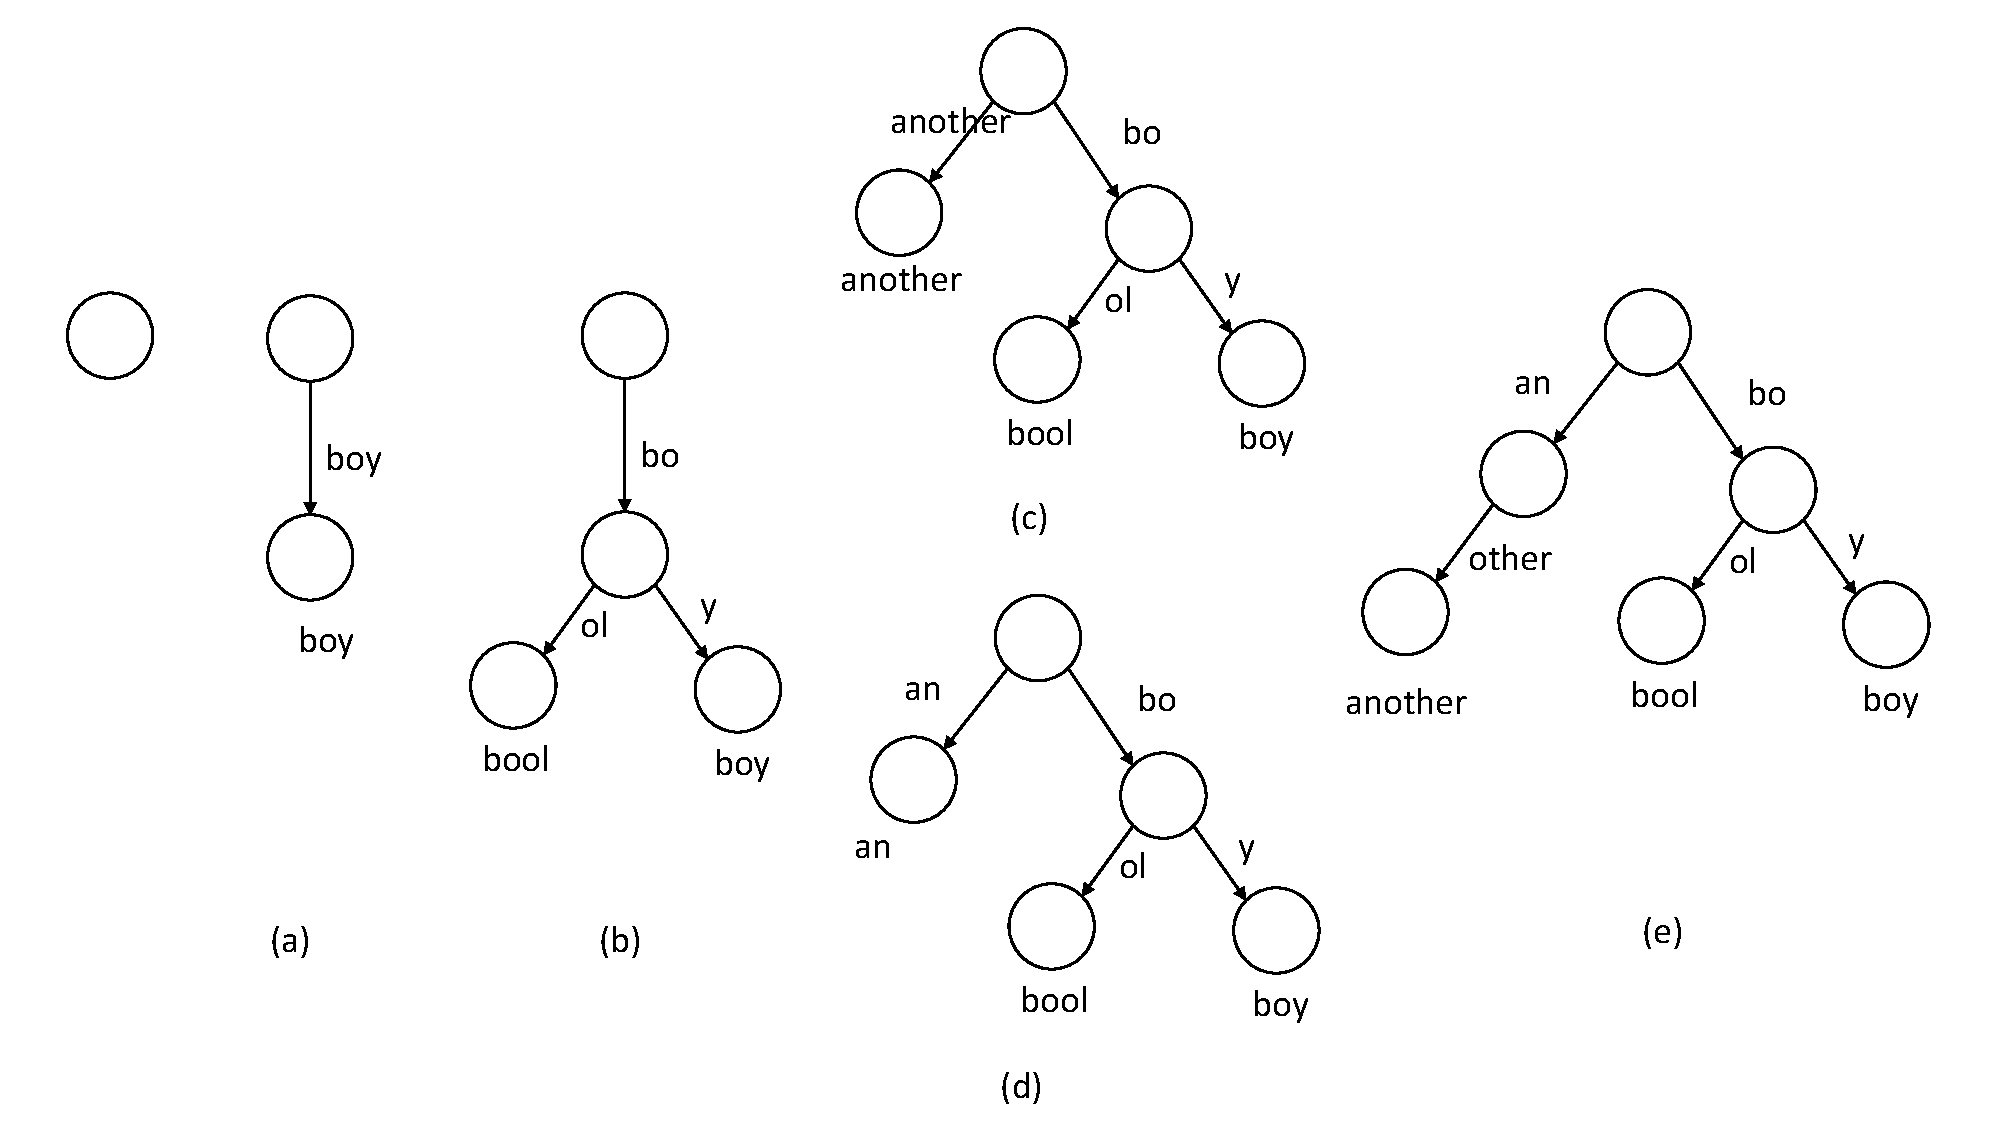
\includegraphics[scale=0.4]{img/prefix-tree-insert}
  \caption{(a) insert `boy' to empty tree; (b) insert `bool', branch a new node out; (c) insert `another' to (b); (d) insert `an' to (b); (e) insert `an' to (c), same result as insert `another' to (d)}
  \label{fig:patricia-insert}
\end{figure}

Below function inserts key $s$ and value $v$ to the prefix tree $t = (v', ts)$:

\be
\begin{array}{rcl}
insert\ [\ ]\ v\ (v', ts) & = & (\textit{Just}\ v, ts) \\
insert\ s\ v\ (v', ts) & = & (v', ins\ ts) \\
\end{array}
\ee

If the key $s$ is empty, we overwrite the value to $v$; otherwise, we call $ins$ to examine the sub-trees and their prefixes.

\be
\begin{array}{rcl}
ins\ [\ ]\ & = & [ s \mapsto (\textit{Just}\ v, [\ ]) ] \\
ins\ ((s' \mapsto t) \cons ts') & = & \begin{cases}
  match\ s\ s': & (branch\ s\ v\ s'\ t) : ts' \\
  \text{otherwise}: & (s' \mapsto t) : ins\ ts' \\
  \end{cases}
\end{array}
\ee

If there is no sub-tree in the node, then we create a leaf of $v$ as the single sub-tree, and map $s$ to it; otherwise, for each sub-tree mapping $s' \mapsto t$, we compare $s'$ with $s$. If they have common prefix (tested by the $match$ function), then we $branch$ out new sub-tree. We define two lists matching if they have common prefix:

\be
\begin{array}{rcl}
match\ [\ ]\ B & = & True \\
match\ A\ [\ ] & = & True \\
match\ (a \cons as)\ (b \cons bs) & = & a = b \\
\end{array}
\ee

To extract the longest common prefix of two lists $A$ and $B$, we define a function $(C, A', B') = lcp\ A\ B$, where $C \doubleplus A' = A$ and $C \doubleplus B' = B$ hold. If either $A$ or $B$ is empty, or their first elements are different, then the common prefix $C = [\ ]$; otherwise, we recursively extract the longest common prefix from the rest lists, and preprend the head element:

\be
\begin{array}{rcl}
lcp\ [\ ]\ B & = & ([\ ], [\ ], B) \\
lcp\ A\ [\ ] & = & ([\ ], A, [\ ]) \\
lcp\ (a \cons as)\ (b \cons bs) & = & \begin{cases}
  a \neq b: & ([\ ], a \cons as, b \cons bs) \\
  \text{otherwise}: & (a \cons cs, as', bs')\\
  \end{cases}
\end{array}
\ee

where $(cs, as', bs') = lcp\ as\ bs$ in the recursive case. Function $branch\ A\ v\ B\ t$ takes two keys $A$, $B$, a value $v$, and a tree $t$. It extracts the longest common prefix $C$ from $A$ and $B$, maps it to a new branch node, and assign sub-trees:

\be
\begin{array}{l}
branch\ A\ v\ B\ t = \\
\ lcp\ A\ B = \begin{cases}
   (C, [\ ], B'): & (C, (\textit{Just}\ v, [B' \mapsto t])) \\
   (C, A', [\ ]): & (C, insert\ A'\ v\ t) \\
   (C, A', B'): & (C, (\textit{Nothing}, [A' \mapsto (\textit{Just}\ v, [\ ]), B' \mapsto t])) \\
\end{cases}
\end{array}
\ee

If $A$ is the prefix of $B$, then $A$ is mapped to the node of $v$, and the remaining list is re-mapped to $t$, which is the single sub-tree in the branch; if $B$ is the prefix of $A$, then we recursively insert the remaining list and the value to $t$; otherwise, we create a leaf node of $v$ put it together with $t$ as the two sub-trees of the branch. The following example program implements the $insert$ algorithm:

\begin{Haskell}
insert [] v (PrefixTree _ ts) = PrefixTree (Just v) ts
insert k v (PrefixTree v' ts) = PrefixTree v' (ins ts) where
    ins [] = [(k, leaf v)]
    ins ((k', t) : ts) | match k k' = (branch k v k' t) : ts
                       | otherwise  = (k', t) : ins ts

leaf v = PrefixTree (Just v) []

match [] _ = True
match _ [] = True
match (a:_) (b:_) = a == b

branch a v b t = case lcp a b of
  (c, [], b') -> (c, PrefixTree (Just v) [(b', t)])
  (c, a', []) -> (c, insert a' v t)
  (c, a', b') -> (c, PrefixTree Nothing [(a', leaf v), (b', t)])

lcp [] bs = ([], [], bs)
lcp as [] = ([], as, [])
lcp (a:as) (b:bs) | a /= b = ([], a:as, b:bs)
                  | otherwise = (a:cs, as', bs') where
                        (cs, as', bs') = lcp as bs
\end{Haskell}

We can eliminate the recursion to implement the $insert$ algorithm in loops.

\begin{algorithmic}[1]
\Function{Insert}{$T, k, v$}
  \If{$T = $ NIL}
   \State $T \gets$ \Call{Empty-Node}{}
  \EndIf
  \State $p \gets T$
  \Loop
    \State $match \gets$ FALSE
    \For{each $s_i \mapsto T_i $ in \Call{Sub-Trees}{$p$}}
      \If{$k = s_i$}
        \State \Call{Value}{$T_i$} $\gets v$ \Comment{Overwrite}
        \State \Return $T$
      \EndIf
      \State $c \gets$ \Call{LCP}{$k, s_i$}
      \State $k_1 \gets k - c$, $k_2 \gets s_i - c$
      \If{$c \neq $ NIL}
        \State $match \gets$ TRUE
        \If{$k_2 = $ NIL} \Comment{$s_i$ is prefix of $k$}
          \State $p \gets T_i$, $k \gets k_1$
          \State break
        \Else \Comment{Branch out a new leaf}
          \State \textproc{Add}(\Call{Sub-Trees}{$p$}, $c \mapsto$ \textproc{Branch}($k_1$, \Call{Leaf}{$v$}, $k_2$, $T_i$))
          \State \textproc{Delete}(\Call{Sub-Trees}{$p$}, $s_i \mapsto T_i$)
          \State \Return $T$
        \EndIf
      \EndIf
    \EndFor
    \If{not $match$} \Comment{Add a new leaf}
      \State \textproc{Add}(\Call{Sub-Trees}{$p$}, $k \mapsto$ \Call{Leaf}{$v$})
      \State break
    \EndIf
  \EndLoop
  \State \Return $T$
\EndFunction
\end{algorithmic}

Function \textproc{LCP} extracts the longest common prefix from two lists.

\begin{algorithmic}[1]
\Function{LCP}{$A, B$}
  \State $i \gets 1 $
  \While{$i \leq |A|$ and $i \leq |B|$ and $A[i] = B[i]$}
    \State $i \gets i + 1$
  \EndWhile
  \State \Return $A[1...i-1]$
\EndFunction
\end{algorithmic}

There is a special case in \textproc{Branch}($s_1, T_1, s_2, T_2$). If $s_1$ is empty, the key to be insert is some prefix. We set $T_2$ as the sub-tree of $T_1$. Otherwise, we create a new branch node and set $T_1$ and $T_2$ as the two sub-trees.

\begin{algorithmic}[1]
\Function{Branch}{$s_1, T_1, s_2, T_2$}
  \If{$s_1 = $ NIL}
    \State \textproc{Add}(\Call{Sub-Trees}{$T_1$}, $s_2 \mapsto T_2$)
    \State \Return $T_1$
  \EndIf
  \State $T \gets$ \Call{Empty-Node}{}
  \State \Call{Sub-Trees}{$T$} $\gets \{s_1 \mapsto T_1, s_2 \mapsto T_2\}$
  \State \Return $T$
\EndFunction
\end{algorithmic}

Although the prefix tree improves the space efficiency of trie, it is still bound to $O(m n)$, where $n$ is the length of the key, and $m$ is the size of the element set.

\subsection{Lookup}
\index{Prefix tree!look up}

When look up a key $k$, we start from the root. If $k = [\ ]$ is empty, then return the root value as the result; otherwise, we examine the sub-tree mappings, locate the one $s_i \mapsto t_i$, such that $s_i$ is some prefix of $k$, then recursively look up $k - s_i$ in sub-tree $t_i$. If there does not exist $s_i$ as the prefix of $k$, then there is no such key in the prefix tree.

\be
\begin{array}{rcl}
lookup\ [\ ]\ (v, ts) & = & v \\
lookup\ k\ (v, ts) & = & find\ ((s, t) \mapsto s \sqsubseteq k)\ ts\ =  \\
  & & \begin{cases}
    \textit{Nothing} : & Nothing \\
    \textit{Just}\ (s, t): & lookup\ (k - s)\ t
  \end{cases}
\end{array}
\ee

Where $A \sqsubseteq B$ means list $A$ is prefix of $B$. Function $find$ is defined in chapter 1, which searches element in a list with a given predication. Below example program implements the look up algorithm.

\begin{Haskell}
lookup [] (PrefixTree v _) = v
lookup ks (PrefixTree v ts) =
  case find (\(s, t) -> s `isPrefixOf` ks) ts of
    Nothing -> Nothing
    Just (s, t) -> lookup (drop (length s) ks) t
\end{Haskell}

The prefix testing is linear to the length of the list, the $lookup$ algorithm is bound to $O(mn)$ time, where $m$ is the size of the element set, and $n$ is the length of the key. We skip the imperative implementation, and leave it as the exercise.

\begin{Exercise}\label{ex:prefix-tr-lookup}
\Question{Eliminate the recursion to implement the prefix tree $lookup$ purely with loops.}
\end{Exercise}

\begin{Answer}[ref = {ex:prefix-tr-lookup}]
\Question{Eliminate the recursion to implement the prefix tree $lookup$ purely with loops.

\begin{Bourbaki}
Optional<V> lookup(PrefixTree<K, V> t, K key) {
    if t == null then return Optional.Nothing
    Bool match
    repeat {
        match = False
        for k, tr in t.subtrees {
            if k == key then return Optional.of(tr.value)
            (K prefix, K k1, K k2) = lcp(key, k)
            if prefix != [] and k2 == [] {
                match = True
                key = k1
                t = tr
                break
            }
        }
    } until not match
    return Optional.Nothing
}
\end{Bourbaki}
}
\end{Answer}

\section{Applications of trie and prefix tree}
We can use trie and prefix tree to solve many interesting problems, like implement a dictionary, populate candidate inputs, and realize the textonym input method. Different from the industry implementation, we give the examples to illustrate the ideas of trie and prefix tree.

\subsection{Dictionary and input completion}
\index{Auto completion}
As shown in \cref{fig:e-dict}, when user enters some characters, the dictionary application searches the library, populates a list of candidate words or phrases that start from what input.

\begin{figure}[htbp]
  \centering
  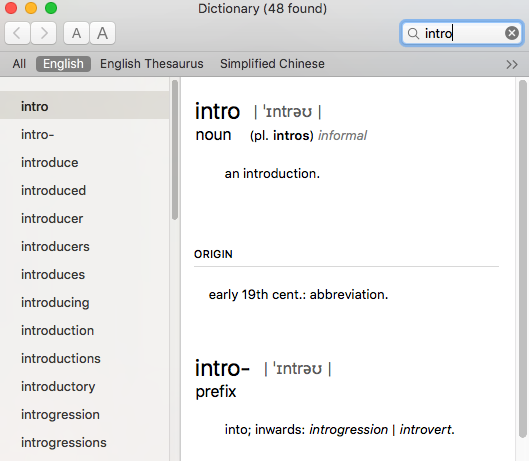
\includegraphics[scale=0.4]{img/edict-en}
  \caption{A dictionary application}
  \label{fig:e-dict}
\end{figure}

A dictionary can contain hundreds of thousands words. It's expensive to perform a complete search. Commercial dictionaries adopt varies engineering approach, like caching, indexing to speed up search. Similarly, \cref{fig:word-completion} shows a smart text input component. When type some characters, it populates a candidate lists, with all items starting with the input string.

\begin{figure}[htbp]
  \centering
  
\includegraphics[scale=0.5]{img/adaptive-input}
  \caption{A smart text input component}
  \label{fig:word-completion}
\end{figure}

Both examples give the `auto-completion' functionality. We can implement it with prefix tree. For illustration purpose, we limit to English characters, and set a upper bound $n$ for the number of candidates. A dictionary stores key-value pairs, where the key is English word or phrase, the value is the corresponding meaning and explanation. When user input string $s$, we look up the prefix tree for all keys start with $s$. If $s$ is empty we expand all sub-trees till reach to $n$ candidates; otherwise, we locate the sub-tree from the mapped key, and look up recursively. In the environment supports lazy evaluation, we can expand all candidates, and take the first $n$ on demand: $take\ n\ (startsWith\ s\ t)$, where $t$ is the prefix tree.

\be
\begin{array}{c}
\begin{array}{rcl}
startsWith\ [\ ]\ (\textit{Nothing}, ts) & = & enum\ ts \\
startsWith\ [\ ]\ (\textit{Just}\ x, ts) & = & ([\ ], x) : enum\ ts \\
startsWith\ s\ (v, ts) & = & find\ ((k, t) \mapsto s \sqsubseteq k\ \text{or}\ k \sqsubseteq s)\ ts = \\
\end{array} \\
\quad \begin{cases}
  \textit{Nothing}: & [\ ] \\
  \textit{Just}\ (k, t): & [(k \doubleplus a, b) | (a, b) \in startsWith\ (s - k)\ t]
\end{cases}
\end{array}
\ee

Given a prefix $s$, function $startsWith$ searches all candidates in the prefix tree starts with $s$. If $s$ is empty, it enumerates all sub-trees, and prepand $([\ ], x)$ for none empty value $x$ in the root. Function $enum\ ts$ is defined as:

\be
enum = \textit{concatMap}\ (k, t) \mapsto [(k \doubleplus a, b) | (a, b) \in startsWith\ [\ ]\ t]
\ee

\label{sec:list-concatmap}
Where $\textit{concatMap}$ (also known as $\textit{flatMap}$) is an important concept for list computation. Literally, it results like firstly map on each element, then concatenate the result together. It's typically realized with 'build-foldr' fusion law to eliminate the intermediate list overhead. (see chapter 5 in my book {\em Isomorphism -- mathematics of programming}) If the input prefix $s$ is not empty, we examine the sub-tree mappings, for each list and sub-tree pair $(k, t)$, if either $s$ is prefix of $k$ or vice versa, we recursively expand $t$ and prepand $k$ to each result key; otherwise, $s$ does not match any sub-trees, hence the result is empty. Below example program implements this algorithm.

\begin{Haskell}
startsWith [] (PrefixTree Nothing ts) = enum ts
startsWith [] (PrefixTree (Just v) ts) = ([], v) : enum ts
startsWith k (PrefixTree _ ts) =
  case find (\(s, t) -> s `isPrefixOf` k || k `isPrefixOf` s) ts of
    Nothing -> []
    Just (s, t) -> [(s ++ a, b) |
                         (a, b) <- startsWith (drop (length s) k) t]

enum = concatMap (\(k, t) -> [(k ++ a, b) | (a, b) <- startsWith [] t])
\end{Haskell}

We can also realize the algorithm \textproc{Starts-With}($T, k, n$) imperatively. From the root, we loop on every sub-tree mapping $k_i \mapsto T_i$. If $k$ is the prefix for any sub-tree $T_i$, we expand all things in it up to $n$ items; if $k_i$ is the prefix of $k$, we then drop that prefix, update the key to $k - k_i$, then search $T_i$ for this new key.

\begin{algorithmic}[1]
\Function{Starts-With}{$T, k, n$}
  \If{$T = $ NIL}
     \State \Return NIL
  \EndIf
  \State $s \gets$ NIL
  \Repeat
    \State $match \gets$ FALSE
    \For{$k_i \mapsto T_i$ in \Call{Sub-Trees}{$T$}}
      \If{$k$ is prefix of $k_i$}
        \State \Return \Call{Expand}{$s \doubleplus k_i, T_i, n$}
      \EndIf
      \If{$k_i$ is prefix of $k$}
        \State $match \gets$ TRUE
        \State $k \gets k - k_i$  \Comment{drop the prefix}
        \State $T \gets T_i$
        \State $s \gets s \doubleplus k_i$
        \State break
      \EndIf
    \EndFor
  \Until{not $match$}
  \State \Return NIL
\EndFunction
\end{algorithmic}

Where function \textproc{Expand}($s, T, n$) populates $n$ results from $T$ and prepand $s$ to each key. We implement it with `breadth first search' method (see section 14.3):

\begin{algorithmic}[1]
\Function{Expand}{$s, T, n$}
  \State $R \gets $ NIL
  \State $Q \gets [(s, T)]$
  \While{$|R| < n$ and $Q \neq$ NIL}
    \State $(k, T) \gets$ \Call{Pop}{$Q$}
    \State $v \gets$ \Call{Value}{$T$}
    \If{$v \neq$ NIL}
      \State \Call{Insert}{$R, (k, v)$}
    \EndIf
    \For{$k_i \mapsto T_i$ in \Call{Sub-Trees}{$T$}}
      \State \Call{Push}{$Q, (k \doubleplus k_i, T_i)$}
    \EndFor
  \EndWhile
\EndFunction
\end{algorithmic}

\subsection{Predictive text input}
\index{T9}

Before 2010, most mobile phones had a small keypad as shown in \cref{fig:itut-keypad}, called ITU-T keypad. It maps a digit to 3 - 4 characters. For example, when input word `home', one can press keys in below sequence:

\begin{figure}[htbp]
  \centering
  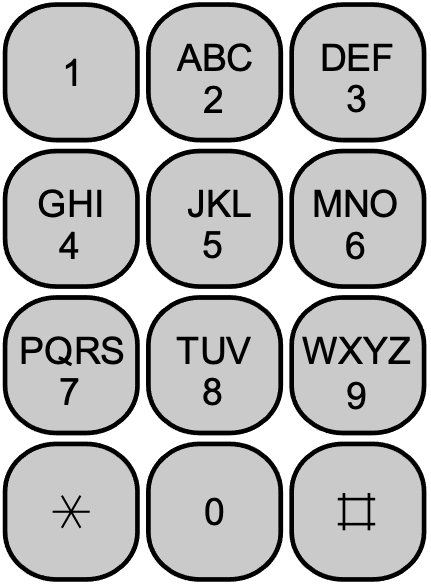
\includegraphics[scale=0.4]{img/itu-t}
  \caption{The mobile phone ITU-T keypad.}
  \label{fig:itut-keypad}
\end{figure}

\begin{enumerate}
\item Press key `4' twice to enter `h';
\item Press key `6' three times to enter `o';
\item Press key `6' to enter  `m';
\item Press key `3' twice to enter `e';
\end{enumerate}

A smarter input method allows to press less keys:

\begin{enumerate}
\item Press key sequence `4', `6', `6', `3', the word `home' appears as a candidate;
\item Press key `*' to change to next candidate, word `good' appears;
\item Press key '*' again for another candidate, word `gone' appears;
\item ...
\end{enumerate}

This is called predictive input, or abbreviated as `T9'\cite{wiki-t9}, \cite {wiki-predictive-text}. We can realize it by storing the word dictionary in a prefix tree. The commercial implementations uses multiple layers of caches/index in both memory and file system. We simplify it as an example of prefix tree application. First, we need define the digit key mappings:

\be
\begin{array}{ll}
M_{T9} = \{ & 2 \mapsto \texttt{"abc"}, 3 \mapsto \texttt{"def"}, 4 \mapsto \texttt{"ghi"}, \\
           & 5 \mapsto \texttt{"jkl"}, 6 \mapsto \texttt{"mno"}, 7 \mapsto \texttt{"pqrs"}, \\
           & 8 \mapsto \texttt{"tuv"}, 9 \mapsto \texttt{"wxyz"} \quad \}
\end{array}
\ee

$M_{T9}[i]$ gives the corresponding characters for digit $i$. We can also define the reversed mapping from a character back to digit.

\be
M^{-1}_{T9} = \textit{concatMap}\ ((d, s) \mapsto [(c, d) | c \in s])\ M_{T9}
\ee

Given a string, we can convert it to a sequence of digits by looking up $M^{-1}_{T9}$.

\be
digits(s) = [ M^{-1}_{T9}[c] | c \in s ]
\ee

For any character does not belong [\texttt{a..z}], we map it to a special key \texttt{'\#'} as fallback. Below example program defines the above two mappings.

\begin{Haskell}
mapT9 = Map.fromList [('2', "abc"), ('3', "def"), ('4', "ghi"),
                      ('5', "jkl"), ('6', "mno"), ('7', "pqrs"),
                      ('8', "tuv"), ('9', "wxyz")]

rmapT9 = Map.fromList $ concatMap (\(d, s) -> [(c, d) | c <- s]) $
           Map.toList mapT9

digits = map (\c -> Map.findWithDefault '#' c rmapT9)
\end{Haskell}

Suppose we already build the prefix tree $(v, ts)$ from all words in a dictionary. We need change the above auto completion algorithm to process digit string $ds$. For every sub-tree mappings $(s \mapsto t) \in ts$, we convert the prefix $s$ to $digits(s)$, check if it matches to $ds$ (either one is the prefix of the other). There can be multiple sub-trees match $ds$ as:

\[
\textit{pfx} = [(s, t) | (s \mapsto t) \in ts, digits(s) \sqsubseteq ds\ \textit{or}\ ds\ \sqsubseteq digits(s)]
\]

\be
\begin{array}{rcl}
find_{T9}\ t\ [\ ] & = & [ [\ ] ] \\
find_{T9}\ (v, ts)\ ds & = & \textit{concatMap}\ find\ \textit{pfx} \\
\end{array}
\ee

For each mapping $(s, t)$ in \textit{pfx}, function $find$ recursively lookup the remaining digits $ds'$ in $t$, where $ds' = drop\ |s|\ ds$, then prepend $s$ to every candidate. However, the length may exceeds the number of digits, we need cut and only take $n = |ds|$ characters:

\be
find\ (s, t) = [ take\ n\ (s \doubleplus s_i) | s_i \in find_{T9}\ t\ ds']
\ee

The following example program implements the predictive input look up algorithm:

\begin{Haskell}
findT9 _ [] = [[]]
findT9 (PrefixTree _ ts) k = concatMap find pfx where
  find (s, t) = map (take (length k) . (s++)) $ findT9 t (drop (length s) k)
  pfx = [(s, t) | (s, t) <- ts, let ds = digits s in
              ds `isPrefixOf` k || k `isPrefixOf` ds]
\end{Haskell} %$

To realize the predictive text input imperatively, we can perform breadth first search with a queue $Q$ of tuples $(\textit{prefix}, D, t)$. Every tuple records the possible \textit{prefix} searched so far; the remaining digits $D$ to be searched; and the sub-tree $t$ we are going to search. $Q$ is initialized with the empty prefix, the whole digits sequence, and the root. We repeatedly pop the tuple from the queue, and examine the sub-tree mappings. for every mapping $(s \mapsto T')$, we convert $s$ to $digits(s)$. If $D$ is prefix of it, then we find a candidate. We append $s$ to \textit{prefix}, and record it in the result. If $digits(s)$ is prefix of $D$, we need further search the sub-tree $T'$. We create a new tuple of $(\textit{prefix} \doubleplus s, D', T')$, where $D'$ is the remaining digits to be searched. Then push this new tuple back to the queue.

\begin{algorithmic}[1]
\Function{Look-Up-T9}{$T, D$}
  \State $R \gets $ NIL
  \If{$T =$ NIL or $D =$ NIL}
    \State \Return $R$
  \EndIf
  \State $n \gets |D|$
  \State $Q \gets \{(\text{NIL}, D, T)\}$
  \While{$Q \neq $ NIL}
    \State $(\textit{prefix}, D, T) \gets$ \Call{Pop}{$Q$}
    \For{$(s \mapsto T') \in $ \Call{Sub-Trees}{$T$}}
      \State $D' \gets$ \Call{Digits}{$s$}
      \If{$D' \sqsubset D$} \Comment{$D'$ is prefix of $D$}
        \State \Call{Append}{$R, (\textit{prefix} \doubleplus s)[1..n]$} \Comment{limit the length to $n$}
      \ElsIf{$D \sqsubset D'$}
        \State \Call{Push}{$Q, (\textit{prefix} \doubleplus s, D - D', T')$}
      \EndIf
    \EndFor
  \EndWhile
  \State \Return $R$
\EndFunction
\end{algorithmic}

We start from integer trie and prefix tree. By turning the integer key to binary format, we re-used binary tree to realize the integer based map data structure. Then extend the key from integer to generic list, and limit the list element to finite set. Particularly for alphabetic strings, the generic trie and prefix tree can be used as tools to manipulate the text information. We give example applications about auto-completion and predictive text input. as another instance of radix tree, the suffix tree is closely related to trie and prefix tree used in text, and DNA processing.

\begin{Exercise}\label{ex:prefix-tree-app}
\Question{Implement the auto-completion and predictive text input with trie.}
\Question{How to ensure the candidates in lexicographic order in the auto-completion and predictive text input program? What's the performance change accordingly?}
\end{Exercise}

\begin{Answer}[ref = {ex:prefix-tree-app}]
\Question{Implement the auto-completion and predictive text input with trie.

For input prefix $ks$, we advance to node $t$ in the trie, expand all sub-trees, the take the first $n$ items:

\begin{Haskell}
import Data.Map (Map)
import qualified Data.Map as Map

startsWith :: Ord k => [k] -> Trie k v -> [([k], v)]
startsWith [] (Trie Nothing  ts) = enum ts
startsWith [] (Trie (Just v) ts) = ([], v) : enum ts
startsWith (k:ks) (Trie _ ts) = case Map.lookup k ts of
  Nothing -> []
  Just t -> map (first (k:)) (startsWith ks t)

enum :: Ord k => Map k (Trie k v) -> [([k], v)]
enum = (concatMap (\(k, t) ->
                    map (first (k:)) (startsWith [] t))) . Map.assocs

get n k t = take n $ startsWith k t
\end{Haskell} %$

Where $\textit{first}\ f\ (a, b) = (f\ a, b)$, it applies the function $f$ to the first one of a pair. When implement predictive input with trie, we lookup $M_{T9}$ for all characters mapped to a digit, then lookup the trie for candidate words.

\begin{Haskell}
findT9 [] _ = [[]]
findT9 (d:ds) (Trie _ ts) = concatMap find cts where
  cts = case Map.lookup d mapT9 of
    Nothing -> []
    Just cs -> Map.assocs $ Map.filterWithKey (\c _ -> c `elem` cs) ts
  find (c, t) = map (c:) (findT9 ds t)
\end{Haskell}
}

\Question{How to ensure the candidates in lexicographic order in the auto-completion and predictive text input program? What's the performance change accordingly?

From exercise \cref{ex:prefix-tree-pre-order-traverse}, if traverse a binary prefix tree in pre-order, the result is in lexicographic order. For multi-way prefix tree, we need traverse sub-trees in lexicographic order. If the sub-trees are managed with self-balanced tree (like the red-black tree or the AVL tree), we can do this in linear time (\cref{ex:bst-iterate}). If the sub-trees are stored in hash table or assoc-list, then we need $O(n \lg n)$ time to sort them.
}
\end{Answer}

\section{Appendix: Example programs}

Definition of integer binary trie:

\begin{lstlisting}[language = Bourbaki]
data IntTrie<T> {
    IntTrie<T> left = null
    IntTrie<T> right = null
    Optional<T> value = Optional.Nothing
}
\end{lstlisting}

The following example $insert$ program uses bit-wise operation to test even/odd, and shift the bit to right:

\begin{lstlisting}[language = Bourbaki]
IntTrie<T> insert(IntTrie<T> t, Int key,
                  Optional<T> value = Optional.Nothing) {
    if t == null then t = IntTrie<T>()
    p = t
    while key != 0 {
        if key & 1 == 0 {
            p = if p.left == null then IntTrie<T>() else p.left
        } else {
            p = if p.right == null then IntTrie<T>() else p.right
        }
        key = key >> 1
    }
    p.value = Optional.of(value)
    return t
}
\end{lstlisting}

%% Integer trie lookup:

%% \begin{lstlisting}[language = Bourbaki]
%% Optional<T> lookup(IntTrie<T> t, Int key) {
%%     while t != null and k != 0 {
%%         t = if key & 1 == 0 then t.left else t.right
%%         key = key >> 1
%%     }
%%     return if t == null then Optional.None else t.value
%% }
%% \end{lstlisting}

Definition of integer prefix tree:

\begin{lstlisting}[language = Bourbaki]
data IntTree<T> {
    Int key
    T value
    Int prefix
    Int mask = 1
    IntTree<T> left = null
    IntTree<T> right = null

    IntTree(Int k, T v) {
        key = k, value = v, prefix = k
    }

    bool isLeaf = (left == null and right == null)

    Self replace(IntTree<T> x, IntTree<T> y) {
        if left == x then left = y else right = y
    }

    bool match(Int k) = maskbit(k, mask) == prefix
}

Int maskbit(Int x, Int mask) = x & (~(mask - 1))
\end{lstlisting}

Insert key-value to integer prefix tree.

\begin{lstlisting}[language = Bourbaki]
IntTree<T> insert(IntTree<T> t, Int key, T value) {
    if t == null then return IntTree(key, value)
    node = t
    Node<T> parent = null
    while (not node.isLeaf()) and node.match(key) {
        parent = node
        node = if zero(key, node.mask) then node.left else node.right
    }
    if node.isleaf() and key == node.key {
        node.value = value
    } else {
        p = branch(node, IntTree(key, value))
        if parent == null then return p
        parent.replace(node, p)
    }
    return t
}

IntTree<T> branch(IntTree<T> t1, IntTree<T> t2) {
    var t = IntTree<T>()
    (t.prefix, t.mask) = lcp(t1.prefix, t2.prefix)
    (t.left, t.right) = if zero(t1.prefix, t.mask) then (t1, t2)
                        else (t2, t1)
    return t
}

bool zero(int x, int mask) = (x & (mask >> 1) == 0)

Int lcp(Int p1, Int p2) {
    Int diff = p1 ^ p2
    Int mask = 1
    while diff != 0 {
        diff = diff >> 1
        mask = mask << 1
    }
    return (maskbit(p1, mask), mask)
}
\end{lstlisting}

%% \begin{lstlisting}[language = Bourbaki]
%% Optional<Node<T>> lookup(Node<T> t, Int key) {
%%     while t != null and (not t.isLeaf()) and t.match(key) {
%%         t = if zero(key, t.mask) then t.left else t.right
%%     }
%%     return if t != null and t.isLeaf() and t.key == key
%%            then Optional.of(t.value) else Optional.None
%% }
%% \end{lstlisting}

Definition of trie and the insert program:

\begin{lstlisting}[language = Bourbaki]
data Trie<K, V> {
  Optional<V> value = Optional.Nothing
  Map<K, Trie<K, V>> subTrees = Map.empty()
}

Trie<K, V> insert(Trie<K, V> t, [K] key, V value) {
    if t == null then t = Trie<K, V>()
    var p = t
    for c in key {
        if p.subTrees[c] == null then p.subTrees[c] = Trie<K, V>()
        p = p.subTrees[c]
    }
    p.value = Optional.of(value)
    return t
}
\end{lstlisting}

Definition of Prefix Tree and insert program:

\begin{lstlisting}[language = Bourbaki]
data PrefixTree<K, V> {
    Optional<V> value = Optional.Nothing
    Map<[K], PrefixTree<K, V>> subTrees = Map.empty()

    Self PrefixTree(V v) {
        value = Optional.of(v)
    }
}

PrefixTree<K, V> insert(PrefixTree<K, V> t, [K] key, V value) {
    if t == null then t = PrefixTree()
    var node = t
    loop {
        bool match = false
        for var (k, tr) in node.subtrees {
            if key == k {
                tr.value = value
                return t
            }
            prefix, k1, k2 = lcp(key, k)
            if prefix != [] {
                match = true
                if k2 == [] {
                    node = tr
                    key = k1
                    break
                } else {
                    node.subtrees[prefix] = branch(k1, PrefixTree(value),
                                                   k2, tr)
                    node.subtrees.delete(k)
                    return t
                }
            }
        }
        if !match {
            node.subtrees[key] = PrefixTree(value)
            break
        }
    }
    return t
}
\end{lstlisting}

The longest common prefix \texttt{lcp} and \texttt{branch} example programs.

\begin{lstlisting}[language = Bourbaki]
([K], [K], [K]) lcp([K] s1, [K] s2) {
    j = 0
    while j < length(s1) and j < length(s2) and s1[j] == s2[j] {
        j = j + 1
    }
    return (s1[0..j-1], s1[j..], s2[j..])
}

PrefixTree<K, V> branch([K] key1, PrefixTree<K, V> tree1,
                        [K] key2, PrefixTree<K, V> tree2) {
    if key1 == []:
        tree1.subtrees[key2] = tree2
        return tree1
    t = PrefixTree()
    t.subtrees[key1] = tree1
    t.subtrees[key2] = tree2
    return t
}
\end{lstlisting}

Populate multiple candidates, they share the common prefix

\begin{lstlisting}[language = Bourbaki]
[([K], V)] startsWith(PrefixTree<K, V> t, [K] key, Int n) {
    if t == null then return []
    [T] s = []
    repeat {
        bool match = false
        for var (k, tr) in t.subtrees {
            if key.isPrefixOf(k) {
                return expand(s ++ k, tr, n)
            } else if k.isPrefixOf(key) {
                match = true
                key = key[length(k)..]
                t = tr
                s = s ++ k
                break
            }
        }
    } until not match
    return []
}

[([K], V)] expand([K] s, PrefixTree<K, V> t, Int n) {
    [([K], V)] r = []
    var q = Queue([(s, t)])
    while length(r) < n and !q.isEmpty() {
        var (s, t) = q.pop()
        v = t.value
        if v.isPresent() then r.append((s, v.get()))
        for k, tr in t.subtrees {
            q.push((s ++ k, tr))
        }
    }
    return r
}
\end{lstlisting}

Predictive text input lookup
\begin{lstlisting}[language = Bourbaki]
var T9MAP={'2':"abc", '3':"def", '4':"ghi", '5':"jkl", \
       '6':"mno", '7':"pqrs", '8':"tuv", '9':"wxyz"}

var T9RMAP = { c : d for var (d, cs) in T9MAP for var c in cs }

string digits(string w) = ''.join([T9RMAP[c] for c in w])

[string] lookupT9(PrefixTree<char, V> t, string key) {
    if t == null or key == "" then return []
    res = []
    n = length(key)
    q = Queue(("", key, t))
    while not q.isEmpty() {
        (prefix, key, t) = q.pop()
        for var (k, tr) in t.subtrees {
            ds = digits(k)
            if key.isPrefixOf(ds) {
                res.append((prefix ++ k)[:n])
            } else if ds.isPrefixOf(key) {
                q.append((prefix ++ k, key[length(k)..], tr))
            }
        }
    }
    return res
}
\end{lstlisting}

\section{Answers}
\shipoutAnswer

\ifx\wholebook\relax \else
\begin{thebibliography}{99}

\bibitem{CLRS}
Thomas H. Cormen, Charles E. Leiserson, Ronald L. Rivest and Clifford Stein.
``Introduction to Algorithms, Second Edition''. Problem 12-1. ISBN:0262032937. The MIT Press. 2001

\bibitem{okasaki-int-map}
Chris Okasaki and Andrew Gill. ``Fast Mergeable Integer
Maps''. Workshop on ML, September 1998, pages 77-86, \url{http://www.cse.ogi.edu/~andy/pub/finite.htm}

\bibitem{patricia-morrison}
D.R. Morrison, ``PATRICIA -- Practical Algorithm To Retrieve  Information Coded In Alphanumeric", Journal of the ACM, 15(4), October 1968, pages 514-534.

\bibitem{wiki-suffix-tree}
Suffix Tree, Wikipedia. \url{https://en.wikipedia.org/wiki/Suffix_tree}

\bibitem{wiki-trie}
Trie, Wikipedia. \url{https://en.wikipedia.org/wiki/Trie}

\bibitem{unplugged}
Xinyu LIU. ``Isomorphism - mathematics of programming''. \url{https://github.com/liuxinyu95/unplugged}

\bibitem{wiki-t9}
T9 (predictive text), Wikipedia. \url{https://en.wikipedia.org/wiki/T9_(predictive_text)}

\bibitem{wiki-predictive-text}
Predictive text,
Wikipedia. \url{https://en.wikipedia.org/wiki/Predictive_text}

\end{thebibliography}

\expandafter\enddocument
\fi
